\documentclass[tikz,border=25pt]{standalone}
\usepackage{tikz}
\usetikzlibrary{shapes, arrows.meta, positioning, fit, backgrounds, calc, shadows, shapes.geometric}
% ===== Academic color palette =====
\definecolor{acaBlueLine}{HTML}{6080B0}      \definecolor{acaBlueFill}{HTML}{DBEAFE}
\definecolor{acaGreenLine}{HTML}{30A060}     \definecolor{acaGreenFill}{HTML}{A0D0A0}
\definecolor{acaOrangeLine}{HTML}{D06020}    \definecolor{acaOrangeFill}{HTML}{FFE6CC}
\definecolor{acaPurpleLine}{HTML}{6020D0}    \definecolor{acaPurpleFill}{HTML}{E1D5E7}
\definecolor{acaRedLine}{HTML}{B05050}       \definecolor{acaRedFill}{HTML}{F8CECC}
\definecolor{acaGreyLine}{HTML}{666666}      \definecolor{acaGreyFill}{HTML}{F5F5F5}
\definecolor{acaGoldLine}{HTML}{D09000}      \definecolor{acaGoldFill}{HTML}{F8F8E0}
\definecolor{acaTealLine}{HTML}{009060}      \definecolor{acaTealFill}{HTML}{D1FAE5}
\definecolor{zoneBlueBg}{HTML}{EEF2FF}
\pgfdeclarelayer{background}
\pgfsetlayers{background,main}
\begin{document}
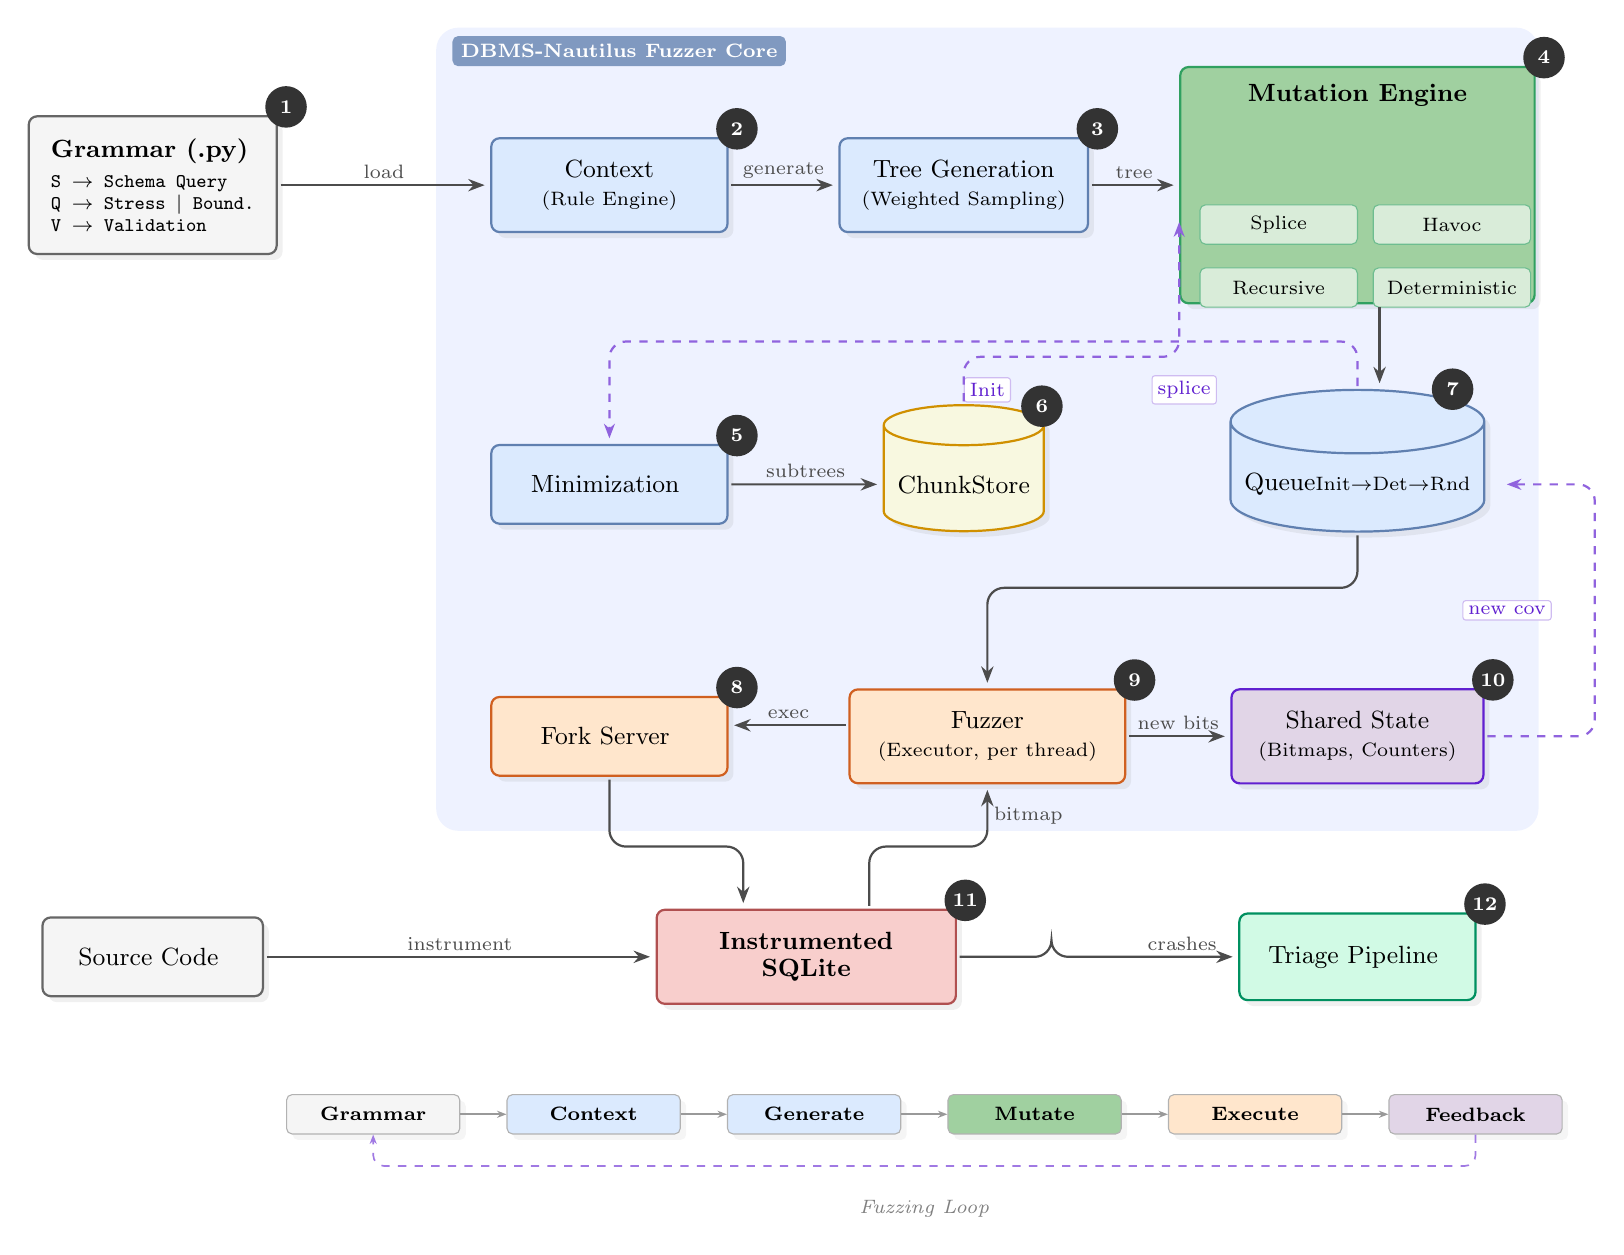
\begin{tikzpicture}[
    every node/.style={font=\small},
    base_box/.style={rectangle, rounded corners=3pt, align=center,
        minimum height=0.9cm, minimum width=2.8cm,
        inner sep=8pt, drop shadow={opacity=0.12}, thick},
    blue_node/.style={base_box, fill=acaBlueFill, draw=acaBlueLine},
    green_node/.style={base_box, fill=acaGreenFill, draw=acaGreenLine},
    orange_node/.style={base_box, fill=acaOrangeFill, draw=acaOrangeLine},
    purple_node/.style={base_box, fill=acaPurpleFill, draw=acaPurpleLine},
    red_node/.style={base_box, fill=acaRedFill, draw=acaRedLine, font=\small\bfseries},
    grey_node/.style={base_box, fill=acaGreyFill, draw=acaGreyLine},
    teal_node/.style={base_box, fill=acaTealFill, draw=acaTealLine},
    subop/.style={rectangle, rounded corners=2pt, draw=acaGreenLine!70,
        fill=acaGreenFill!40, minimum width=2.0cm, minimum height=0.5cm,
        font=\scriptsize, inner sep=3pt, align=center},
    num/.style={circle, fill=black!80, text=white, font=\scriptsize\bfseries,
        inner sep=0pt, minimum size=15pt},
    arrow/.style={-{Stealth[scale=0.9]}, thick, color=black!70,
        shorten >=2pt, shorten <=1pt},
    feedarrow/.style={-{Stealth[scale=0.8]}, thick, dashed, color=acaPurpleLine!70,
        shorten >=2pt, shorten <=1pt},
    tag/.style={font=\scriptsize, inner sep=2pt},
    tagbg/.style={font=\scriptsize, inner sep=2pt, fill=white, rounded corners=1pt, draw=black!10},
    fbtag/.style={font=\scriptsize, inner sep=2pt, fill=white, rounded corners=1pt, draw=acaPurpleLine!30, text=acaPurpleLine},
    stagelbl/.style={fill=acaBlueLine!80, text=white, font=\scriptsize\bfseries,
        rounded corners=2pt, inner sep=3pt},
]
    % ═══════════════════════════════════════════
    % ROW 1 (y=11): Grammar → Context → TreeGen → Mutation
    % ═══════════════════════════════════════════
    \node[grey_node, minimum width=3.0cm, minimum height=1.6cm, align=left,
        font=\scriptsize\ttfamily] (grammar) at (-2.8, 11) {
        \textrm{\small\bfseries Grammar (.py)}\\[3pt]
        S $\to$ Schema Query\\
        Q $\to$ Stress $|$ Bound.\\
        V $\to$ Validation
    };
    \node[blue_node, minimum width=3.0cm, minimum height=1.1cm] (context) at (3.0, 11) {
        Context\\[-1pt]{\scriptsize (Rule Engine)}
    };
    \node[blue_node, minimum width=3.0cm, minimum height=1.1cm] (treegen) at (7.5, 11) {
        Tree Generation\\[-1pt]{\scriptsize (Weighted Sampling)}
    };
    % HERO: Mutation Engine
    \node[green_node, minimum width=4.5cm, minimum height=3.0cm,
        inner sep=10pt] (mutation) at (12.5, 11) {};
    \node[font=\small\bfseries, anchor=north] at ([yshift=-3pt]mutation.north) {Mutation Engine};
    \node[subop] at ([xshift=-1.0cm, yshift=-0.5cm]mutation.center) {Splice};
    \node[subop] at ([xshift=1.2cm, yshift=-0.5cm]mutation.center) {Havoc};
    \node[subop] at ([xshift=-1.0cm, yshift=-1.3cm]mutation.center) {Recursive};
    \node[subop] at ([xshift=1.2cm, yshift=-1.3cm]mutation.center) {Deterministic};
    % ═══════════════════════════════════════════
    % ROW 2 (y=7.2): Minimization, ChunkStore, Queue
    % ═══════════════════════════════════════════
    \node[blue_node, minimum width=3.0cm, minimum height=1.0cm] (mini) at (3.0, 7.2) {
        Minimization
    };
    \node[cylinder, draw=acaGoldLine, fill=acaGoldFill, thick,
        shape border rotate=90, minimum height=1.6cm, minimum width=1.2cm,
        aspect=0.25, inner sep=5pt, font=\small,
        drop shadow={opacity=0.12}] (chunkstore) at (7.5, 7.2) {
        Chunk\\[-1pt]Store
    };
    \node[cylinder, draw=acaBlueLine, fill=acaBlueFill, thick,
        shape border rotate=90, minimum height=1.8cm, minimum width=1.4cm,
        aspect=0.25, inner sep=5pt, font=\small,
        drop shadow={opacity=0.12}] (queue) at (12.5, 7.2) {
        Queue\\[-2pt]{\scriptsize Init$\to$Det$\to$Rnd}
    };
    % ═══════════════════════════════════════════
    % ROW 3 (y=4.0): ForkServer, Fuzzer, SharedState
    % ═══════════════════════════════════════════
    \node[orange_node, minimum width=3.0cm, minimum height=1.0cm] (forkserver) at (3.0, 4.0) {
        Fork Server
    };
    \node[orange_node, minimum width=3.5cm, minimum height=1.1cm] (fuzzer) at (7.8, 4.0) {
        Fuzzer\\[-1pt]{\scriptsize (Executor, per thread)}
    };
    \node[purple_node, minimum width=3.2cm, minimum height=1.1cm] (shared) at (12.5, 4.0) {
        Shared State\\[-1pt]{\scriptsize (Bitmaps, Counters)}
    };
    % ═══════════════════════════════════════════
    % ROW 4 (y=1.2): Source, SQLite, Triage
    % ═══════════════════════════════════════════
    \node[grey_node, minimum width=2.8cm, minimum height=1.0cm] (source) at (-2.8, 1.2) {
        Source Code
    };
    \node[red_node, minimum width=3.8cm, minimum height=1.1cm] (sqlite) at (5.5, 1.2) {
        Instrumented\\[-1pt]SQLite
    };
    \node[teal_node, minimum width=3.0cm, minimum height=1.1cm] (triage) at (12.5, 1.2) {
        Triage Pipeline
    };
    % ═══════════════════════════════════════════
    % NUMBER BADGES
    % ═══════════════════════════════════════════
    \node[num] at ([xshift=3pt, yshift=3pt]grammar.north east) {1};
    \node[num] at ([xshift=3pt, yshift=3pt]context.north east) {2};
    \node[num] at ([xshift=3pt, yshift=3pt]treegen.north east) {3};
    \node[num] at ([xshift=3pt, yshift=3pt]mutation.north east) {4};
    \node[num] at ([xshift=3pt, yshift=3pt]mini.north east) {5};
    \node[num] at ([xshift=3pt, yshift=3pt]chunkstore.north east) {6};
    \node[num] at ([xshift=3pt, yshift=3pt]queue.north east) {7};
    \node[num] at ([xshift=3pt, yshift=3pt]forkserver.north east) {8};
    \node[num] at ([xshift=3pt, yshift=3pt]fuzzer.north east) {9};
    \node[num] at ([xshift=3pt, yshift=3pt]shared.north east) {10};
    \node[num] at ([xshift=3pt, yshift=3pt]sqlite.north east) {11};
    \node[num] at ([xshift=3pt, yshift=3pt]triage.north east) {12};
    % ═══════════════════════════════════════════
    % ZONE BACKGROUND
    % ═══════════════════════════════════════════
    \begin{pgfonlayer}{background}
        \fill[zoneBlueBg, rounded corners=8pt]
            (0.8, 2.8) rectangle (14.8, 13.0);
    \end{pgfonlayer}
    \node[stagelbl, anchor=north west] at (1.0, 12.9) {DBMS-Nautilus Fuzzer Core};
    % ═══════════════════════════════════════════
    % ARROWS — Clean routing, no overlaps, no boxes-pierced
    % ═══════════════════════════════════════════
    % --- Forward data flow (top row, left→right) ---
    \draw[arrow] (grammar.east) -- (context.west)
        node[tag, above, midway] {load};
    \draw[arrow] (context.east) -- (treegen.west)
        node[tag, above, midway] {generate};
    \draw[arrow] (treegen.east) -- (mutation.west)
        node[tag, above, midway] {tree};
    % --- Mutation → Queue (down, offset right so it does NOT collide with F1) ---
    \draw[arrow]
        ([xshift=8pt]mutation.south) -- ([xshift=8pt]mutation.south |- queue.north);
    % --- Queue → Fuzzer
    % Route: down from queue, left along y=5.4 (between rows 2 and 3), into fuzzer.north
    \draw[arrow, rounded corners=6pt]
        (queue.south) -- ([yshift=-0.7cm]queue.south)
        -| (fuzzer.north);
    % --- Fuzzer ↔ ForkServer (paired arrows, offset vertically so they don't overlap) ---
    \draw[arrow]
        ([yshift=4pt]fuzzer.west) -- ([yshift=4pt]forkserver.east)
        node[tag, above, midway] {exec};
    % --- ForkServer → SQLite (drop down from forkserver, into sqlite top from above-left) ---
    \draw[arrow, rounded corners=6pt]
        (forkserver.south) -- (forkserver.south |- {(0,2.6)})
        -| ([xshift=-0.8cm]sqlite.north);
    % --- SQLite → Fuzzer (bitmap, route up the right side of SQLite, then up to fuzzer.south) ---
    \draw[arrow, rounded corners=6pt]
        ([xshift=0.8cm]sqlite.north) -- ([xshift=0.8cm]sqlite.north |- {(0,2.6)})
        -| (fuzzer.south)
        node[tag, right, pos=0.75] {bitmap};
    % --- Fuzzer → SharedState (right) ---
    \draw[arrow] (fuzzer.east) -- (shared.west)
        node[tag, above, midway] {new bits};
    % --- Storage connections ---
    \draw[arrow] (mini.east) -- (chunkstore.west)
        node[tag, above, midway] {subtrees};
    % --- External connections ---
    \draw[arrow] (source.east) -- (sqlite.west)
        node[tag, above, midway] {instrument};
    % --- SQLite → Triage (crashes) — route AROUND fuzzer/shared via the bottom-right ---
    \draw[arrow, rounded corners=6pt]
        (sqlite.east) -- ($(sqlite.east) + (1.2,0)$)
        |- (triage.west)
        node[tag, above, pos=0.85] {crashes};
    % ═══════════════════════════════════════════
    % FEEDBACK LOOPS (dashed purple)
    % ═══════════════════════════════════════════
    % F1: SharedState → Queue (new coverage)
    % Route up the far-right rail so it doesn't collide with A4 (Mutation→Queue)
    \draw[feedarrow, rounded corners=6pt]
        (shared.east) -- ($(shared.east) + (1.4,0)$)
        |- ([xshift=0.2cm]queue.east);
    \node[fbtag] at (14.4, 5.6) {new cov};
    % F2: Queue → Mini (Init items go to minimizer)
    % Route ABOVE row 2 to avoid passing through ChunkStore
    \draw[feedarrow, rounded corners=6pt]
        (queue.north) -- ([yshift=0.6cm]queue.north)
        -- ([yshift=0.6cm]queue.north -| mini.north) -- (mini.north);
    \node[fbtag] at (7.8, 8.4) {Init};
    % F3: ChunkStore → Mutation (splice material)
    % Route up the left side of mutation, entering at mutation.west (above all sub-boxes)
    \draw[feedarrow, rounded corners=6pt]
        (chunkstore.north) -- ([yshift=0.6cm]chunkstore.north)
        -| ([yshift=-0.4cm]mutation.west);
    \node[fbtag] at (10.3, 8.4) {splice};
    % ═══════════════════════════════════════════
    % PIPELINE SUMMARY BAR
    % ═══════════════════════════════════════════
    \node[fill=acaGreyFill, draw=black!30, rounded corners=2pt,
          minimum width=2.2cm, minimum height=0.5cm,
          font=\scriptsize\bfseries, drop shadow={opacity=0.08}]
        (pGrammar) at (0, -0.8) {Grammar};
    \node[fill=acaBlueFill, draw=black!30, rounded corners=2pt,
          minimum width=2.2cm, minimum height=0.5cm,
          font=\scriptsize\bfseries, drop shadow={opacity=0.08}]
        (pContext) at (2.8, -0.8) {Context};
    \node[fill=acaBlueFill, draw=black!30, rounded corners=2pt,
          minimum width=2.2cm, minimum height=0.5cm,
          font=\scriptsize\bfseries, drop shadow={opacity=0.08}]
        (pGenerate) at (5.6, -0.8) {Generate};
    \node[fill=acaGreenFill, draw=black!30, rounded corners=2pt,
          minimum width=2.2cm, minimum height=0.5cm,
          font=\scriptsize\bfseries, drop shadow={opacity=0.08}]
        (pMutate) at (8.4, -0.8) {Mutate};
    \node[fill=acaOrangeFill, draw=black!30, rounded corners=2pt,
          minimum width=2.2cm, minimum height=0.5cm,
          font=\scriptsize\bfseries, drop shadow={opacity=0.08}]
        (pExecute) at (11.2, -0.8) {Execute};
    \node[fill=acaPurpleFill, draw=black!30, rounded corners=2pt,
          minimum width=2.2cm, minimum height=0.5cm,
          font=\scriptsize\bfseries, drop shadow={opacity=0.08}]
        (pFeedback) at (14.0, -0.8) {Feedback};
    \foreach \a/\b in {pGrammar/pContext, pContext/pGenerate, pGenerate/pMutate,
        pMutate/pExecute, pExecute/pFeedback} {
        \draw[-{Stealth[scale=0.6]}, semithick, color=black!40]
            (\a.east) -- (\b.west);
    }
    % Pipeline feedback loop — drop BELOW the pipeline bar so it doesn't clip anything above
    \draw[-{Stealth[scale=0.6]}, semithick, color=acaPurpleLine!60, dashed,
        rounded corners=4pt]
        (pFeedback.south) -- ++(0, -0.4) -| (pGrammar.south);
    \node[font=\scriptsize\itshape, color=black!50] at (7.0, -2.0) {Fuzzing Loop};
\end{tikzpicture}
\end{document}